\documentclass{handout_utfpr}

\usepackage[brazil]{babel}
\usepackage{xcolor}
\usepackage{pbox}

\newcommand{\com}[1]{
        \colorbox{gray}{\texttt{\pbox{2cm}{\$ #1}}}
}

\handoutdate{\today}

\begin{document}
\maketitle
\section{Introdução}

Este material é apresentado como parte de uma série de minicursos que serão ministrados sobre tópicos variados com o intuito de \textit{nivelar} o conhecimento dos alunos com relação a conceitos básicos que não estão inclusos nas ementas das disciplinas regulares do curso, bem como colocá-los em contato com ferramentas úteis e boas práticas da Computação.

Os conteúdos são dispostos aqui apenas como um apanhado geral com o objetivo de prover um embasamento mínimo e recomenda-se que outras fontes de pesquisa sejam utilizadas para o aprofundamento nestes assuntos.

\subsection{Unix}
O sistema \textbf{Unix} é um sistema operacional desenvolvido por Ken Thompson, Dennis Richie, Douglas McIlroy e Joe Ossanna em 1970, na American Telephone \& Telegraph Company (AT\&T).

Este sistema foi projetado para ser portável, multi-tarefa e multi-usuário. Sistemas Unix são caracterizados por vários conceitos, como o uso de arquivos de texto para guardar dados, um sistema de arquivos hierárquico, o tratamento de certos dispositivos como arquivos (sec tal) e a idéia de que é melhor ter vários programas pequenos, cada um desempenhando uma única tarefa, de forma que eles possam ser encadeados para realizar uma tarefa maior do que o uso de um só programa que possua todas as funcionalidades. Estes conceitos são conhecidos como a ``filosofia Unix''.

% que permitia uma grande portabilidade para diversas plataformas, o que fez com que o sistema crescesse rapidamente e fosse muito utilizado por instituições academicas. O sistema Unix gerou a criação do projeto GNU por Richard Stallman.

% Under Unix, the operating system consists of many utilities along with the master control program, the kernel. The kernel provides services to start and stop programs, handles the file system and other common "low level" tasks that most programs share, and schedules access to avoid conflicts when programs try to access the same resource or device simultaneously. To mediate such access, the kernel has special rights, reflected in the division between user-space and kernel-space.

\subsection{Tanenbaum e o MINIX}
Em 1987, Andrew S. Tanenbaum, enquanto professor da Vrije Universiteit em Amsterdã, desenvolveu o \textbf{MINIX} (mini-Unix), um sistema que seguia os mesmos princípios do Unix mas que seria usado somente propósitos educacionais, como material de apoio ao seu livro ``Operating Systems: Design and Implementation'' (em português: ``Sistemas Operacionais: Projeto e Implementação'').

Os princípios aplicados por Tanenbaum no MINIX, influenciaram um de seus alunos, Linus Torvalds quando da criação de seu próprio sistema operacional, que mais tarde se tornaria o kernel do \textbf{Linux}.

% No final do desenvolvimento de seu sistema, Linus compartilhou em um fórum o que havia feito:

% \emph{Hello everybody out there using minix -
% I'm doing a (free) operating system (just a hobby, won't be big and professional like gnu) for 386(486) AT clones. This has been brewing since april, and is starting to get ready. I'd like any feedback on things people like/dislike in minix, as my OS resembles it somewhat (same physical layout of the file-system (due to practical reasons) among other things).

% I've currently ported bash(1.08) and gcc(1.40), and things seem to work. This implies that I'll get something practical within a few months, and I'd like to know what features most people would want. Any suggestions are welcome, but I won't promise I'll implement them :-)
% Linus (torvalds@kruuna.helsinki.fi)

% PS. Yes – it's free of any minix code, and it has a multi-threaded fs. It is NOT portable (uses 386 task switching etc), and it probably never will support anything other than AT-harddisks, as that's all I have :-(.

% —Linus Torvalds}

\section{Conhecendo o Linux}

\subsection{GNU/Linux}
blabvlabla gnu

\subsection{O kernel}
O kernel é a parte do sistema que faz a ponte entre os recursos de \textit{hardware}, como CPU, dispositivos de entrada e saída e memória; e a camada de \textit{software}.

Numa configuração monolítica (Linux, Windows, etc), os programas rodam em ``espaço de usuário'', o que significa que um programa usa apenas o espaço de memória reservado a ele e não possui acesso direto a recursos do sistema. Para que um programa efetue uma ação como por exemplo exibir uma mensagem na tela, é necessário que uma ``chamada de sistema'' seja feita através do kernel, já que o programa não tem acesso à placa gráfica do computador.

A figura a seguir exemplifica a arquitetura básica de um sistema Linux:
\begin{figure}[!h]
  \centering
  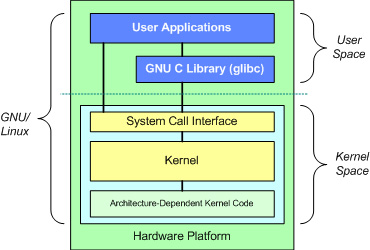
\includegraphics[scale=.8]{kernel.jpg}
  \caption{Arquitetura de um sistema GNU/Linux}
  \label{fig:kernel}
\end{figure}
Na camada superior, em espaço de usuário, estão as aplicações de usuário e a biblioteca GNU. Estas aplicações interagem com o kernel através de uma interface de chamadas de sistema. O kernel, por sua vez, faz acesso ao hardware.

\subsection{Distribuições}

\subsection{}


\subsection{Como obter?}

\subsubsection{Virtual Machine}
Uma máquina virtual (\textbf{VM}) é um computador fictício, baseado somente em \emph{software}. A VM funciona como um emulador, reproduzindo a arquitetura e funcionalidades de um computador de verdade.
Instalar o Linux em uma VM garante a utilização de programas e aplicações como se instalássemos direto no computador, entretanto diminuindo a eficiência, já que estamos tentando utilizar um sistema operacional a partir de outro.


\end{document}
